\section{Transpose}
\label{sec:transpose}

We present three algorithms for optimizing the transpose matrix operation in this section.

The serial code for a transpose operation is presented in \cref{lst:transpose seq}.
The code loops through each index of the input, \ttt{h\_in[i,j]}, and copies the value to the transposed index in the output, \ttt{h\_out[j,i]}.
Given $n=\mathtt{width}$, $m=\mathtt{height}$ this algorithm will have a workload of $\mathcal{O}(nm)$ and step size of $\mathcal{O}(nm)$.

\begin{lstlisting}[caption={Serial transpose}, label={lst:transpose seq}]
void map(int *h_in, int *h_out, const int ROWS, const int COLUMNS) {
for(int row=0; row < ROWS; row++)
  for(int column=0; column < COLUMNS; column++)
    out[column + row*COLUMNS] = in[row + column*ROWS];
}
\end{lstlisting}

As we can analyse the problem as a mapping operation, which we introduced in \cref{sec:challenges with parallel programs}, we know that mapping operations are independent from one another why the amount of steps can be reduced to $\mathcal{O}(1)$ and the problem thus becomes 100\% parallelisible.
In \cref{lst:transpose elem} we present a trivial elem-wise parallel implementation of the transpose algorithm.

\begin{lstlisting}[caption={Parallel transpose}, label={lst:transpose elem}]
__global__
void transpose_kernel(int * d_out, int * d_in,
                      const int ROWS, const int COLUMNS){
  int row = threadIdx.x + blockIdx.x * blockDim.x;
  int column = threadIdx.y + blockIdx.y * blockDim.y;
  if((row >= ROWS) || (column >= COLUMNS)) return;
  d_out[column + row*COLUMNS] = d_in[row + column*ROWS];
}
\end{lstlisting}

The dilemma with the trivial element-wise transpose presented in \cref{lst:transpose elem} is that the kernel will read row-wise but write column-wise.
The row-wise read will utilize coalesced reading whereas the writes will not be coalesced resulting in only one write per bus, wasting $48-4=44$ bytes.
To utilize coalesced writes we present the tiled transpose exemplified in \cref{fig:tiled transpose} and implemented in \cref{lst:transpose tiled}.
The tiled transpose uses shared memory to make coalesced writes to global memory, such as introduced in \cref{sec:shared memory}.

\begin{figure}[htb]
\centering
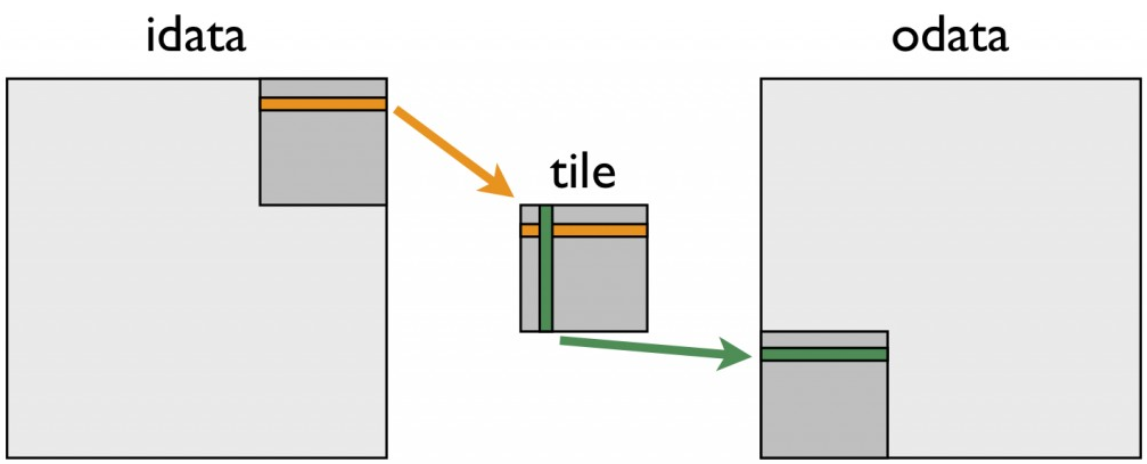
\includegraphics[width=.8\textwidth]{images/transpose-example.png}
\caption{Tiled transpose example}
\label{fig:tiled transpose}
\end{figure}

\begin{lstlisting}[caption={Tiled transpose implementation}, label={lst:transpose tiled}]
__global__
void transpose_kernel_tiled(int * d_out, int * d_in,
                            const int ROWS, const int COLUMNS){
  __shared__ int tile[DIM][DIM]; 
  int x = threadIdx.x + blockIdx.x * blockDim.x,
      y = threadIdx.y + blockIdx.y * blockDim.y;
  if((x >= COLUMNS) || (y >= ROWS)) return;
  tile[threadIdx.y][threadIdx.x] = d_in[x + y*COLUMNS];
  __syncthreads();
  x = threadIdx.x + blockIdx.y * blockDim.y;
  y = threadIdx.y + blockIdx.x * blockDim.x;
  d_out[x + y*ROWS] = tile[threadIdx.x][threadIdx.y];
}
\end{lstlisting}

The tiled solution, however, has memory bank conflicts such as described in \cref{sec:bank conflicts}.
To avert bank conflicts we convert line \ttt{4} to \ttt{tile[DIM][DIM+1]}.
The speed-ups are presented in \cref{tab:transpose speed-ups} for a problem of size $n=2^{14}$, $m=2^{14}$.

\begin{table}[htb]
  \centering
  \begin{tabular}{c r | r r r r}
    \toprule
    device & algorithm & time in ms & speed-up & bandwidth usage & usage percentage\\
    \midrule
    {CPU} & serial  & 6288.88 &  &  &  \\
    \multirow{3}*{GPGPU} & elem-wise & 33.61 & x187.11 & 63.89 GB/s & 22.16\% \\
                         & tiled & 24.93  & x252.26 & 86.14 GB/s & 29.87\% \\
                         & tiled+bank & 16.99 & x370.15 & 126.40 GB/s & 43.83\% \\
    \bottomrule
  \end{tabular}
  \caption{Global vs. Shared memory read and writes}
  \label{tab:transpose speed-ups}
\end{table}

It is to be noted that we could not get the tiled and tiled+bank to run a successful transpose if the input matrix was not a square and if the \ttt{BLOCK\_SIZE} was not able to cover the matrix without overlapping blocks (e.g. threads out of bounds).
We tried using online communities for this issue as described in \cref{sec:help}, but unfortunately did not get any responses.
